%%% PyKEEN hierarchical extensions overview — figure for the 4-page ISWC poster-track paper.
%%% Four columns mirror the paper's paragraph headings, in pipeline order
%%% (data -> task -> model -> metric): Datasets & Analytics, Evaluation Tasks,
%%% Embedding Models, Link Prediction Metrics. Gray chips are stock PyKEEN
%%% components; blue chips are our contributions; the dashed chip marks future work.
\documentclass[tikz,border=0pt]{standalone}
\usepackage{amsmath,amssymb}
\usepackage[T1]{fontenc}
\usetikzlibrary{arrows.meta, positioning, shapes.misc, calc, backgrounds, fit}

% ── Colour palette (project-wide) ───────────────────────────────────────
\definecolor{varblue}{HTML}{3B82F6}
\definecolor{uriteal}{HTML}{0D9488}
\definecolor{wingreen}{HTML}{059669}
\definecolor{costamber}{HTML}{D97706}
\definecolor{edgegray}{HTML}{475569}
\definecolor{titledark}{HTML}{1E293B}
\definecolor{levelbox}{HTML}{94A3B8}
\definecolor{blankslate}{HTML}{64748B}
\definecolor{panelbg}{HTML}{F8FAFC}
\definecolor{querybg}{HTML}{F1F5F9}
\definecolor{entcoral}{HTML}{F87171}
\definecolor{entviolet}{HTML}{8B5CF6}
\definecolor{entamber}{HTML}{F59E0B}

\begin{document}
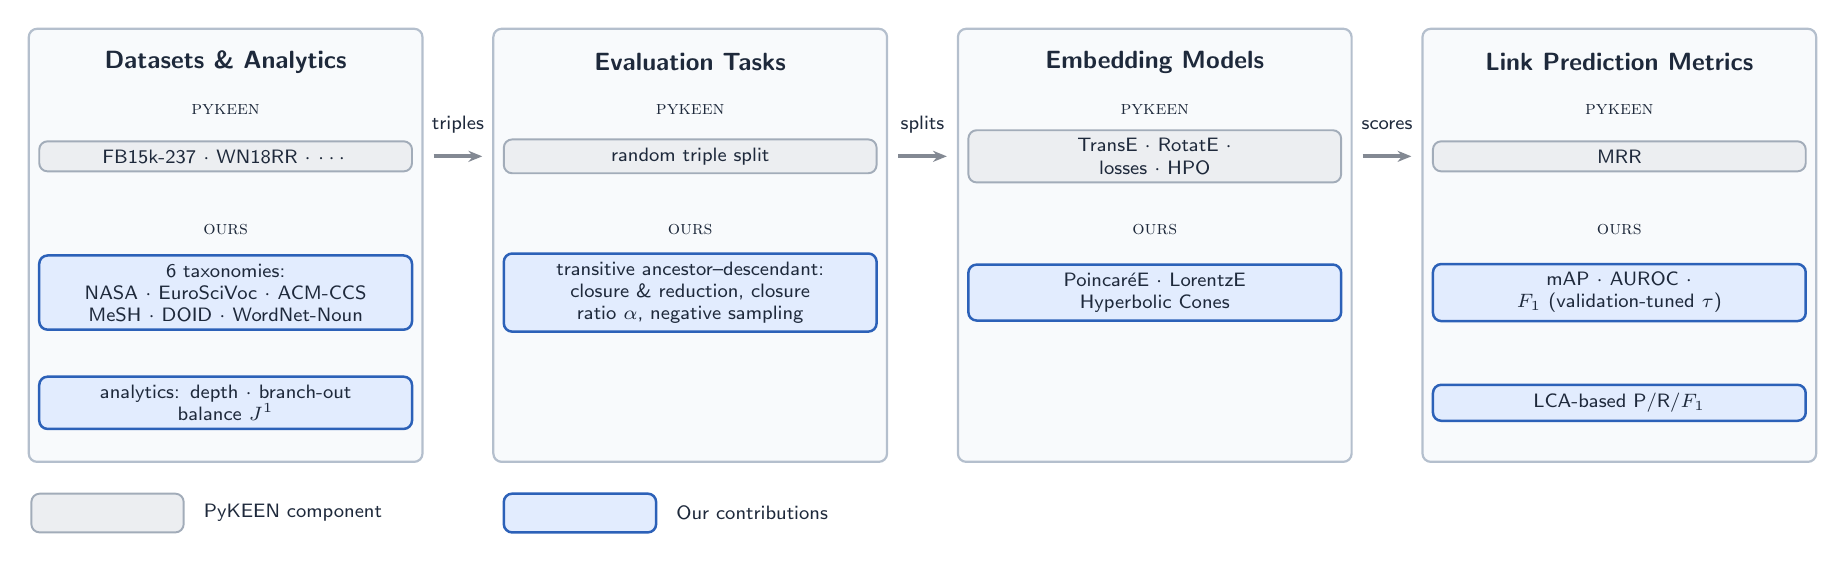
\begin{tikzpicture}[
    font=\sffamily,
    >={Stealth[length=5pt, width=4pt]},
    % ── shared styles ──
    panel label/.style={font=\footnotesize\sffamily\scshape, text=edgegray},
    sub label/.style={font=\scriptsize\sffamily, text=titledark},
    inner box/.style={draw=levelbox!70, line width=0.8pt, rounded corners=3pt,
        fill=panelbg},
    module title/.style={font=\small\sffamily\bfseries\scshape, text=titledark},
    group label/.style={font=\scriptsize\sffamily\scshape, text=titledark},
    pyk chip/.style={draw=blankslate!60, fill=blankslate!12, rounded corners=3pt,
        line width=0.7pt, font=\scriptsize\sffamily, text=titledark,
        align=center, inner ysep=3pt, text width=#1},
    hp chip/.style={draw=varblue!75!black, fill=varblue!15, rounded corners=3pt,
        line width=0.9pt, font=\scriptsize\sffamily, text=titledark,
        align=center, inner ysep=3pt, text width=#1},
    future chip/.style={draw=varblue!60, dash pattern=on 3pt off 2pt,
        rounded corners=3pt, line width=0.9pt, font=\scriptsize\sffamily,
        text=titledark, align=center, inner ysep=3pt, text width=#1},
    flow arrow/.style={->, draw=edgegray!70, line width=1pt},
    transition/.style={draw=titledark!55, line width=1.4pt, ->,
        shorten <=4pt, shorten >=4pt},
    tlabel/.style={font=\scriptsize\sffamily, text=titledark, align=center},
]

% ══════════════════════════════════════════════════════════════════════
%  DIMENSIONS — four columns mirroring the paper's paragraph headings
% ══════════════════════════════════════════════════════════════════════
\def\panelT{0}    \def\panelB{-5.5}
\def\rowA{-1.62}  \def\rowB{-3.35}  \def\rowC{-4.75}   % chip row centres
\def\DL{0}    \def\DR{5.0}    \def\Dcx{2.5}    % Datasets & Analytics
\def\PL{5.9}  \def\PR{10.9}   \def\Pcx{8.4}    % Evaluation Tasks
\def\LL{11.8} \def\LR{16.8}   \def\Lcx{14.3}   % Embedding Models
\def\EL{17.7} \def\ER{22.7}   \def\Ecx{20.2}   % Link Prediction Metrics
\def\chipW{4.5cm}

% ══════════════════════════════════════════════════════════════════════
%  PANEL FRAMES + TITLES
% ══════════════════════════════════════════════════════════════════════
\begin{scope}[on background layer]
  \draw[inner box] (\DL,\panelB) rectangle (\DR,\panelT);
  \draw[inner box] (\PL,\panelB) rectangle (\PR,\panelT);
  \draw[inner box] (\LL,\panelB) rectangle (\LR,\panelT);
  \draw[inner box] (\EL,\panelB) rectangle (\ER,\panelT);
\end{scope}

\node[module title] at (\Dcx,-0.42) {Datasets \& Analytics};
\node[module title] at (\Pcx,-0.42) {Evaluation Tasks};
\node[module title] at (\Lcx,-0.42) {Embedding Models};
\node[module title] at (\Ecx,-0.42) {Link Prediction Metrics};

% ══════════════════════════════════════════════════════════════════════
%  DATASETS & ANALYTICS
% ══════════════════════════════════════════════════════════════════════
\node[group label] at (\Dcx,-1.02) {pykeen};
\node[pyk chip=\chipW] at (\Dcx,\rowA) {FB15k-237 $\cdot$ WN18RR $\cdot$ $\cdots$};
\node[group label] at (\Dcx,-2.55) {ours};
\node[hp chip=\chipW] at (\Dcx,\rowB)
    {6 taxonomies:\\NASA $\cdot$ EuroSciVoc $\cdot$ ACM-CCS\\MeSH $\cdot$ DOID $\cdot$ WordNet-Noun};
\node[hp chip=\chipW] at (\Dcx,\rowC)
    {analytics: depth $\cdot$ branch-out\\balance $J^1$};

% ══════════════════════════════════════════════════════════════════════
%  EVALUATION TASKS  (task band folded in as the pipeline's task stage)
% ══════════════════════════════════════════════════════════════════════
\node[group label] at (\Pcx,-1.02) {pykeen};
\node[pyk chip=\chipW] at (\Pcx,\rowA) {random triple split};
\node[group label] at (\Pcx,-2.55) {ours};
\node[hp chip=\chipW] at (\Pcx,\rowB)
    {transitive ancestor--descendant:\\closure \& reduction, closure\\ratio $\alpha$, negative sampling};

% ══════════════════════════════════════════════════════════════════════
%  EMBEDDING MODELS
% ══════════════════════════════════════════════════════════════════════
\node[group label] at (\Lcx,-1.02) {pykeen};
\node[pyk chip=\chipW] at (\Lcx,\rowA)
    {TransE $\cdot$ RotatE $\cdot$\\losses $\cdot$ HPO};
\node[group label] at (\Lcx,-2.55) {ours};
\node[hp chip=\chipW] at (\Lcx,\rowB)
    {Poincar\'eE $\cdot$ LorentzE\\Hyperbolic Cones};

% ══════════════════════════════════════════════════════════════════════
%  LINK PREDICTION METRICS
% ══════════════════════════════════════════════════════════════════════
\node[group label] at (\Ecx,-1.02) {pykeen};
\node[pyk chip=\chipW] at (\Ecx,\rowA) {MRR};
\node[group label] at (\Ecx,-2.55) {ours};
\node[hp chip=\chipW] at (\Ecx,\rowB)
    {mAP $\cdot$ AUROC $\cdot$\\$F_1$ (validation-tuned $\tau$)};
\node[hp chip=\chipW] at (\Ecx,\rowC) {LCA-based P/R/$F_1$};

% ══════════════════════════════════════════════════════════════════════
%  FLOW ARROWS between columns  (data -> task -> model -> metric)
% ══════════════════════════════════════════════════════════════════════
\draw[transition] (\DR,\rowA) -- (\PL,\rowA);
\node[tlabel] at ({(\DR+\PL)/2},-1.22) {triples};
\draw[transition] (\PR,\rowA) -- (\LL,\rowA);
\node[tlabel] at ({(\PR+\LL)/2},-1.22) {splits};
\draw[transition] (\LR,\rowA) -- (\EL,\rowA);
\node[tlabel] at ({(\LR+\EL)/2},-1.22) {scores};

% ══════════════════════════════════════════════════════════════════════
%  LEGEND
% ══════════════════════════════════════════════════════════════════════
\node[pyk chip=1.7cm] at (1.0,-6.15) {\strut};
\node[sub label, anchor=west] at (2.1,-6.15) {PyKEEN component};
\node[hp chip=1.7cm] at (7.0,-6.15) {\strut};
\node[sub label, anchor=west] at (8.1,-6.15) {Our contributions};

\end{tikzpicture}
\end{document}
